\lab{Pandas 2: Plotting}{Pandas 2: Plotting}
\objective{Clear, insightful visualizations are a crucial part of data analysis.
To facilitate quick data visualization, pandas includes several tools that wrap around matplotlib.
These tools make it easy to compare different parts of a data set and explore the data as a whole.
}

\section*{Overview of Plotting Tools} % =======================================

The main tool for visualization in pandas is the \li{plot()} method of the \li{Series} and \li{DataFrame}.
The method has a keyword argument \li{kind} that specifies the type of plot to draw.
The valid options for \li{kind} are detailed below.

\begin{table}[H]
\begin{tabular}{r|c|l}
Plot Type & \li{plot()} ID & Uses and Advantages \\ \hline
Line plot & \li{"line"} & Show trends ordered in data; easy to compare multiple data sets \\
Scatter plot & \li{"scatter"} & Compare exactly two data sets, independent of ordering \\
Bar plot & \li{"bar"}, \li{"barh"} & Compare categorical or sequential data \\
Histogram & \li{"hist"} & Show frequencies of one set of values, independent of ordering \\
% Kernel Density Estimation & \li{"kde"} & Estimate a smooth distribution \\
Box plot & \li{"box"} & Display min, median, max, and quartiles; compare data distributions \\
Hexbin plot & \li{"hexbin"} & 2D histogram; reveal density of cluttered scatter plots \\
\end{tabular}
\caption{Uses for the \li{plot()} method of the pandas \li{Series} and \li{DataFrame}.
The plot ID is the value of the keyword argument \li{kind}.
That is, \li{df.plot(kind="scatter")} creates a scatter plot.
The default \li{kind} is \li{"line"}.}
\label{table:pandas-plot-options}
\end{table}

The \li{plot()} method calls \li{plt.plot()}, \li{plt.hist()}, \li{plt.scatter()}, or another matplotlib plotting function, but it also assigns axis labels, tick marks, legends, and a few other things based on the index and the data.
Most calls to \li{plot()} specify the \li{kind} of plot and which \li{Series} to use as the \li{x} and \li{y} axes.
By default, the \li{index} of the \li{Series} or \li{DataFrame} is used for the \li{x} axis.

% In Pandas, a \li{DataFrame} is an ordered collection of \li{Series}.
% A Series is similar to a dictionary, with values assigned to various labels, or indices.
% Each Series becomes a column in the data frame, with each row corresponding to an index.
% When several Series are combined into a single data frame, it becomes very easy to compare and visualize data.
% Each entry has an associated index and column.

\begin{lstlisting}
>>> import pandas as pd
>>> from matplotlib import pyplot as plt

>>> crime = pd.read_csv("crime_data.csv", index_col="Year")
>>> crime.plot(y="Population")  # Plot population against the index (years).
\end{lstlisting}

\begin{figure}[H]
\centering
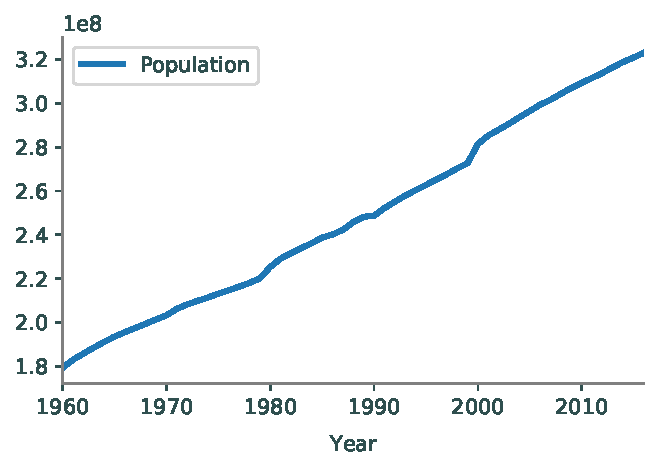
\includegraphics[width=.7\textwidth]{figures/population.pdf}
\end{figure}

In this case, the call to the \li{plot()} method is essentially equivalent to the following code.

\begin{lstlisting}
>>> plt.plot(crime.index, crime["Population"], label="Population")
>>> plt.xlabel(crime.index.name)
>>> plt.xlim(min(crime.index), max(crime.index))
>>> plt.legend(loc="best")
\end{lstlisting}

The \li{plot()} method also takes in many keyword arguments for matplotlib plotting and annotation functions.
For example, setting \li{legend=False} disables the legend, providing a value for \li{title} sets the figure title, \li{grid=True} turns a grid on, and so on.
For more customizations, see \url{https://pandas.pydata.org/pandas-docs/stable/generated/pandas.DataFrame.plot.html}.

\subsection*{Visualizing an Entire Data Set} % --------------------------------

A good way to start analyzing an unfamiliar data set is to visualize as much of the data as possible to determine which parts are most important or interesting.
For example, since the columns in a \li{DataFrame} share the same index, the columns can all be graphed together using the index as the $x$-axis.
In fact, the \li{plot()} method attempts by default to plot \textbf{every} \li{Series} (column) in the \li{DataFrame}.
This is especially useful with sequential data, like the crime data set.

The crime data set has 11 columns, so the resulting figure, Figure \ref{fig:crime-all}, is fairly cluttered.
However, it does shows that the \li{"Population"} column is on a completely different scale than the others.
Dropping a few columns gives a better overview of the data, shown in Figure \ref{fig:crime-all-v2}.

\begin{lstlisting}
# Plot all columns together against the index.
>>> crime.plot(linewidth=1)

# Plot all columns together except for 'Population' and 'Total'.
>>> crime.drop(["Population", "Total"], axis=1).plot(linewidth=1)
\end{lstlisting}

\begin{figure}[H] % Plot everything together.
\captionsetup[subfigure]{justification=centering}
\centering
\begin{subfigure}{.49\textwidth}
    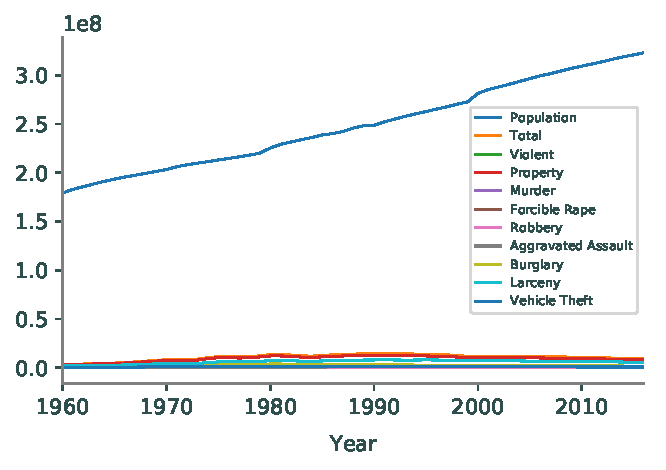
\includegraphics[width=\textwidth]{figures/all_crime.pdf}
    \caption{All columns of the crime data set on the same figure, using the index as the $x$-axis.}
    \label{fig:crime-all}
\end{subfigure}
%
\begin{subfigure}{.49\textwidth}
    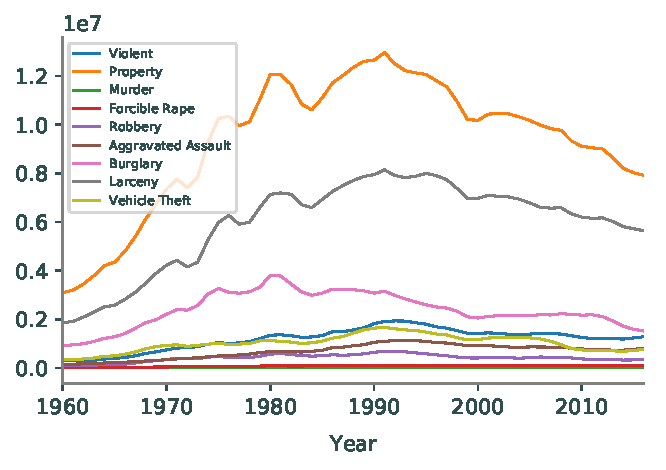
\includegraphics[width=\textwidth]{figures/all_crime2.pdf}
    \caption{All columns of the crime data set except \li{"Population"} and \li{"Total"}.}
    \label{fig:crime-all-v2}
\end{subfigure}
\caption{}
\end{figure}

\begin{warn}
The \li{"Population"} column differs from the other columns because it is has \textbf{different units of measure}: population is measured by ``number of people,'' but all other columns are measured in ``number of crimes.''
Be careful not to plot parts of a data set together if those parts don't have the same units or are otherwise incomparable.
\end{warn}

To quickly plot several columns in separate subplots, use \li{subplots=True} and specify a shape tuple as the \li{layout} for the plots.
Subplots automatically share the same $x$-axis; set \li{sharey=True} to force them to share the same $y$-axis as well.

\begin{lstlisting}
>>> crime.plot(y=["Property", "Larceny", "Burglary", "Violent"],
...            subplots=True, layout=(2,2), sharey=True,
...            style=['-', '--', '-.', ':'])
\end{lstlisting}

\begin{figure}[H]
    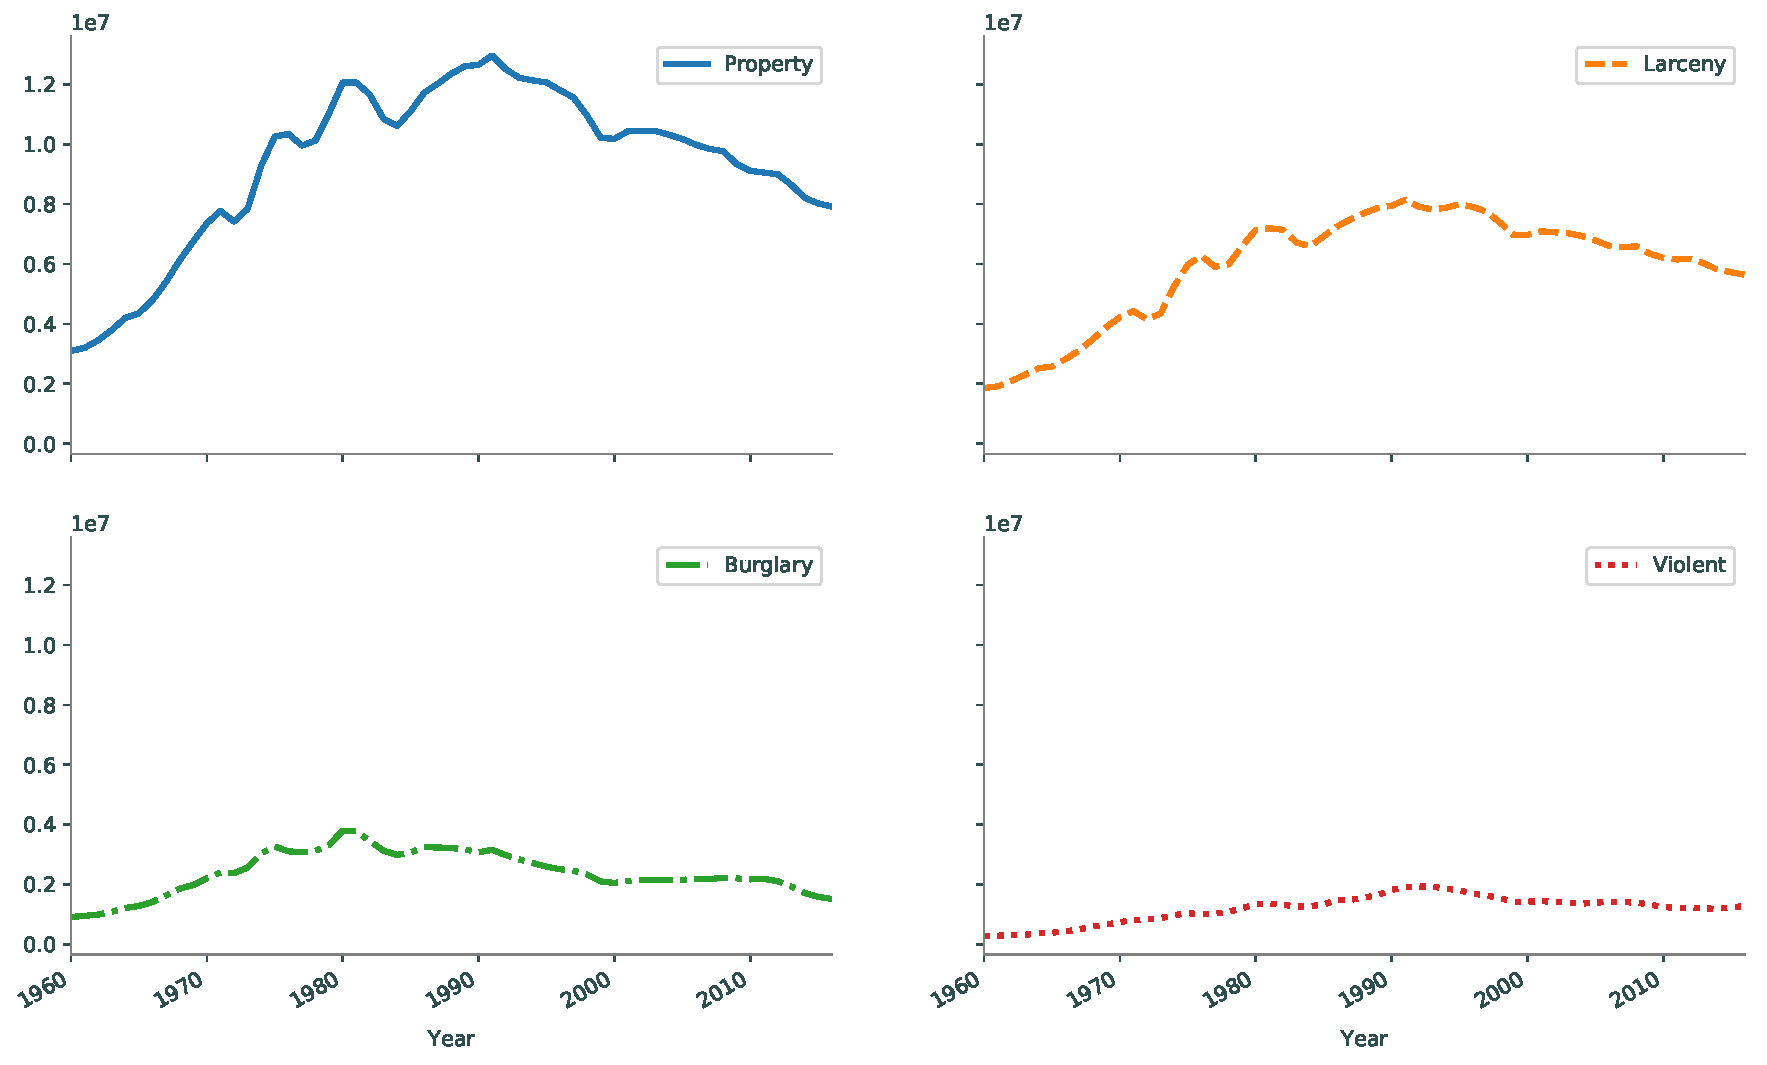
\includegraphics[width=.7\textwidth]{figures/line_subplots.pdf}
\end{figure}

The \li{plot()} method can generate subplots of any kind of plot.
However, since subplots share an $x$-axis by default, histograms turn out poorly whenever there are columns with very different data ranges.
For histograms, use the \li{hist()} method of the \li{DataFrame} instead of the \li{plot()} method.
Specify the number of bins with the \li{bins} parameter.

\begin{lstlisting}
>>> crime[["Violent","Murder","Robbery","Property"]].hist(grid=False, bins=20)
\end{lstlisting}

\begin{figure}[H]
    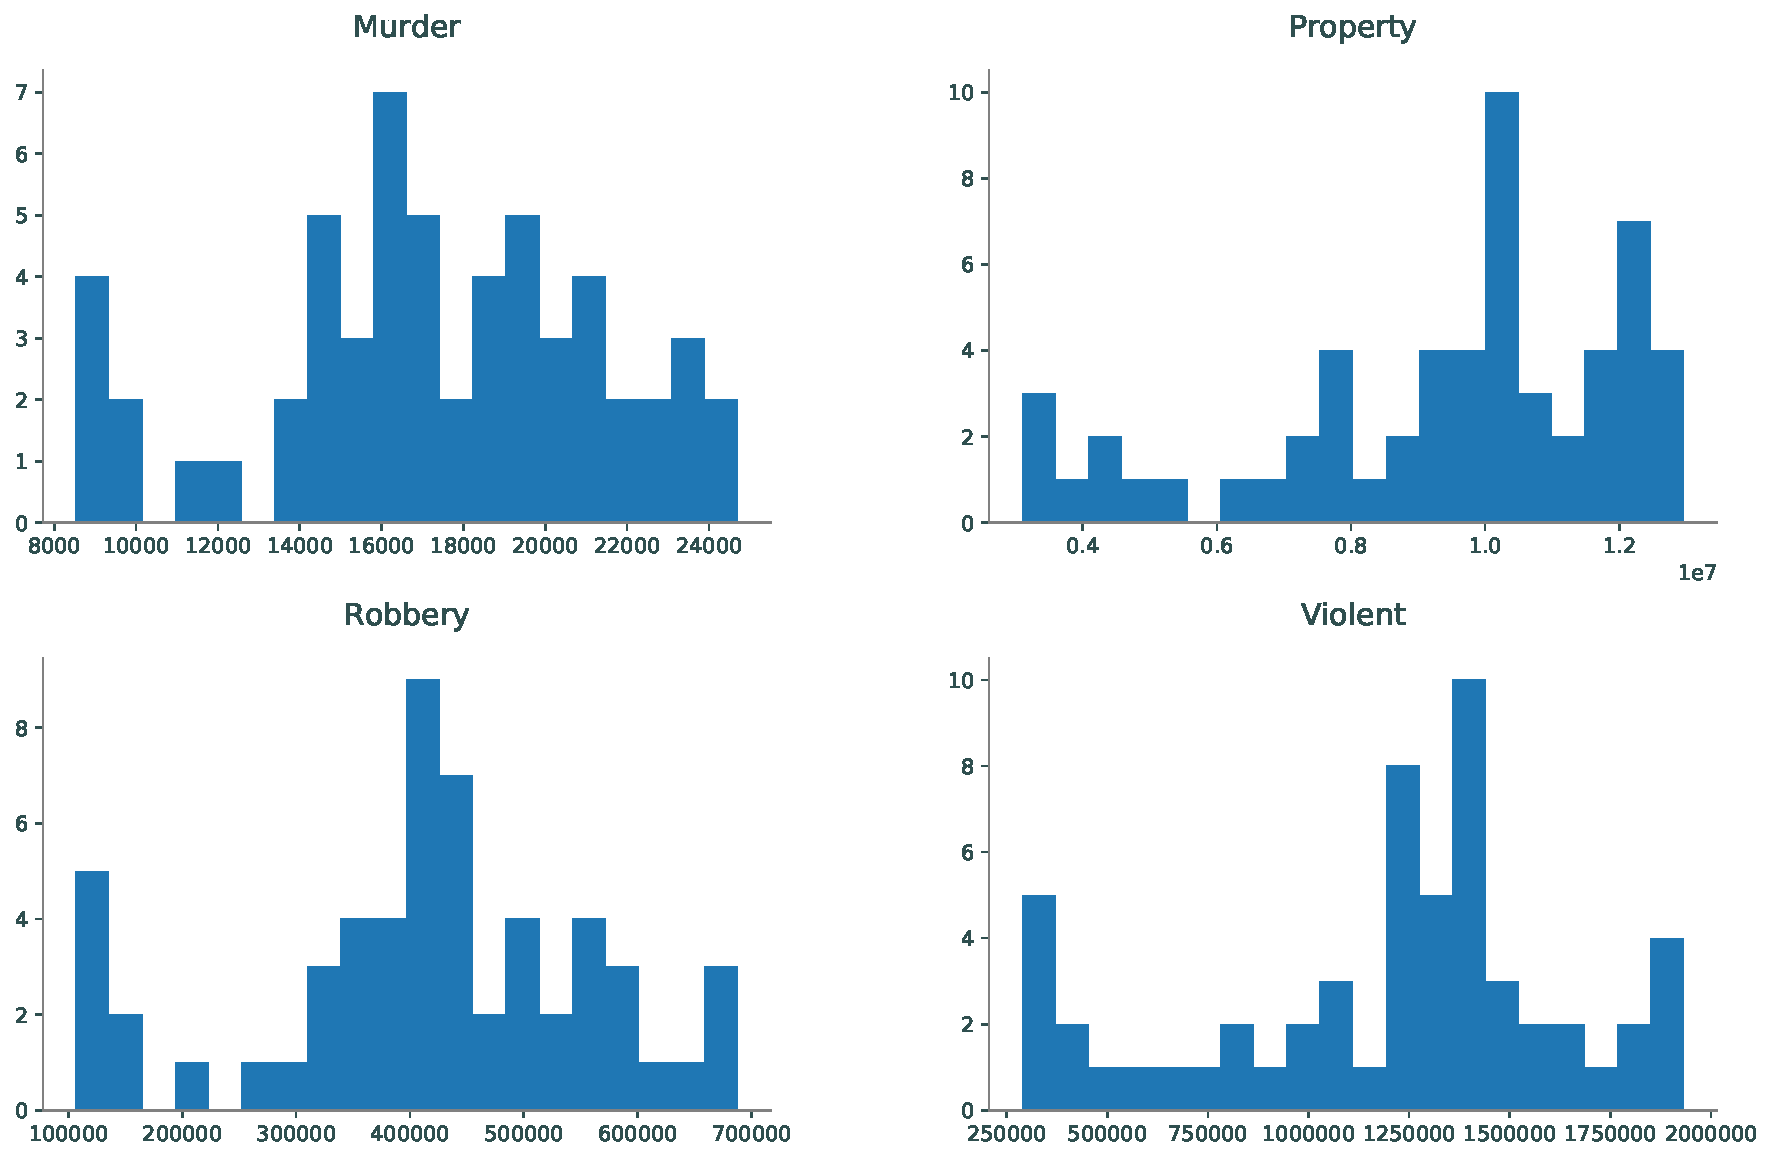
\includegraphics[width=.7\textwidth]{figures/hist_subplots.pdf}
\end{figure}

Finally, the function \li{pd.plotting.scatter_matrix()} produces a table of plots where each column is plotted against each other column in separate scatter plots.
The plots on the diagonal, instead of plotting a column against itself, displays a histogram of that column.
This provides a way to very quickly do an initial analysis of the correlation between different columns.

\begin{lstlisting}
>>> pd.plotting.scatter_matrix(crime[["Population", "Total", "Violent"]])
\end{lstlisting}

\begin{figure}[H]
    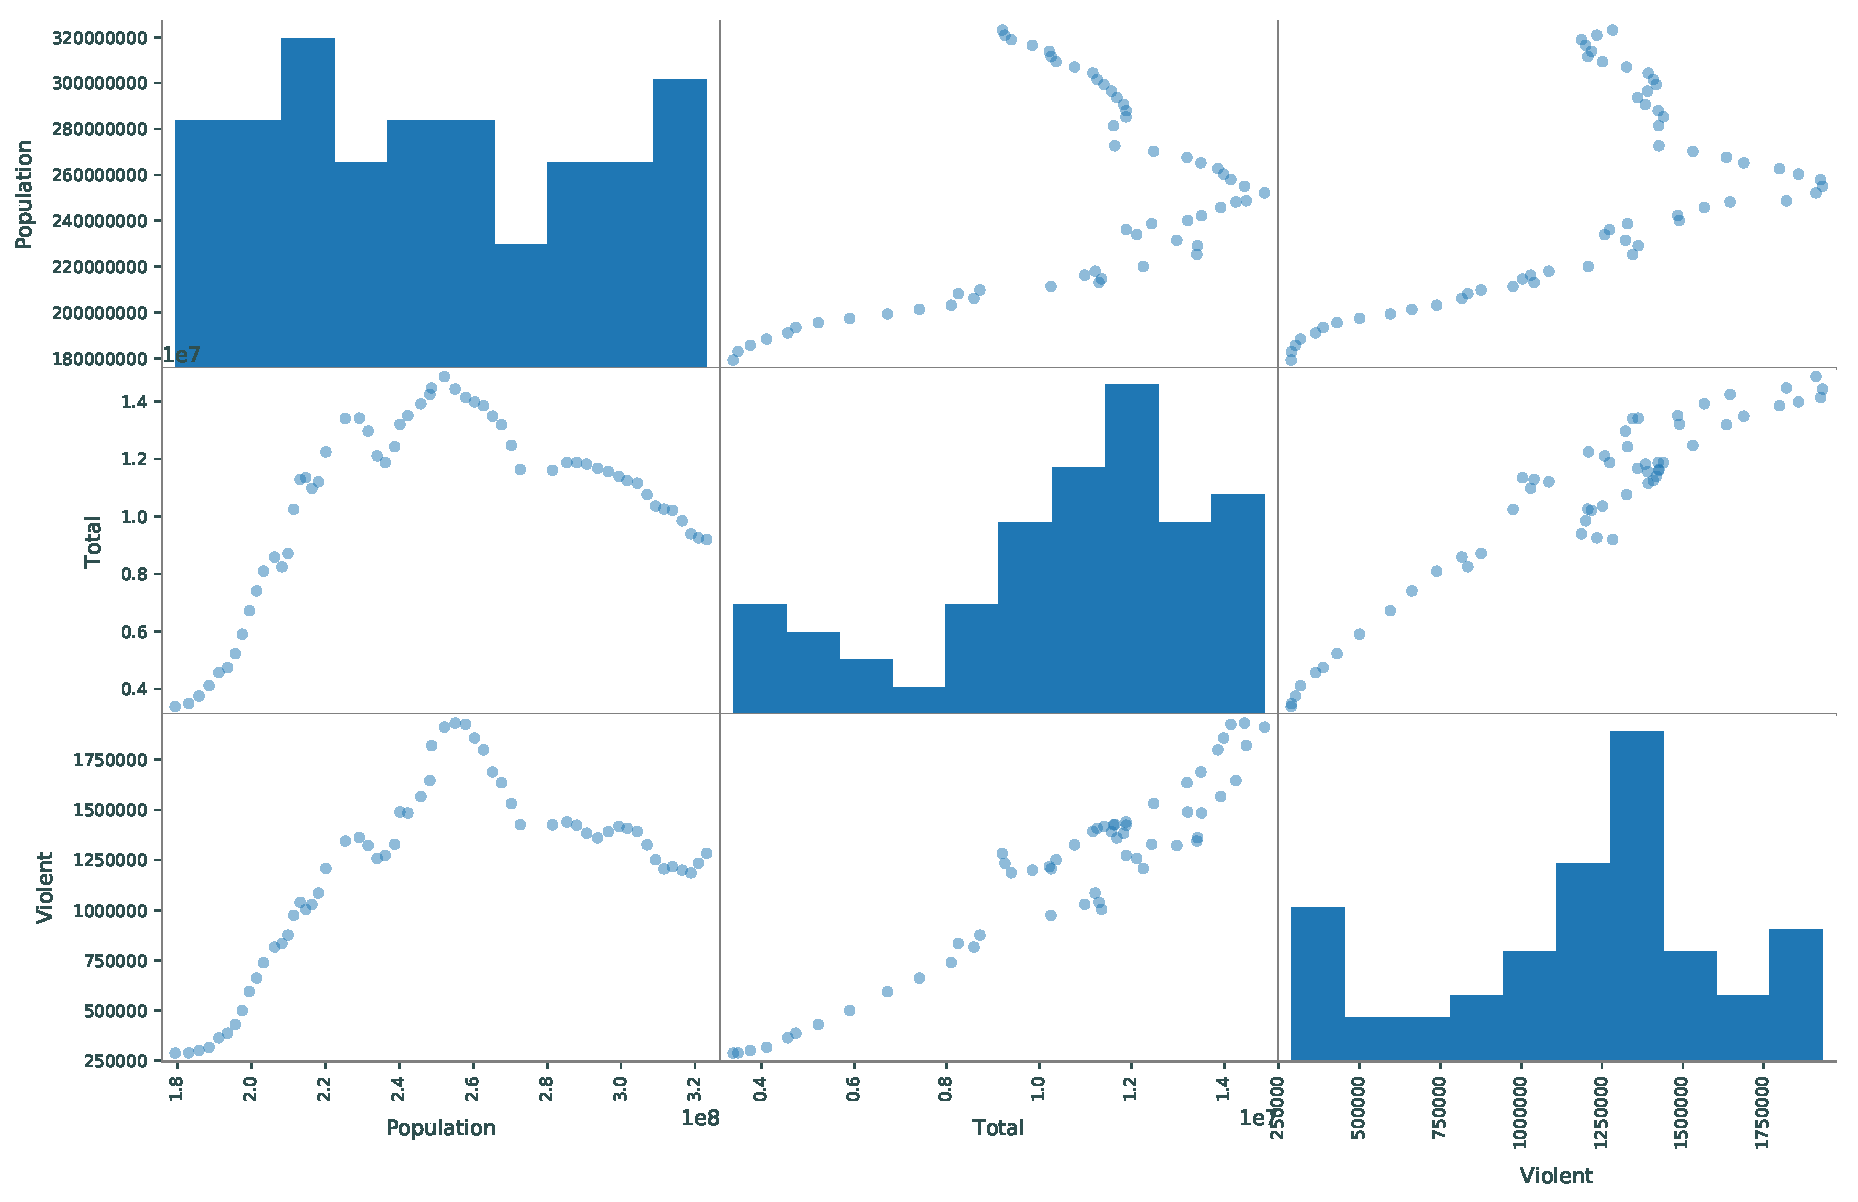
\includegraphics[width=.7\textwidth]{figures/scatter_table.pdf}
\end{figure}

\section*{Patterns and Correlations} % ========================================

After visualizing the entire data set initially, the next step is usually to closely compare related parts of the data.
For example, Figure \ref{fig:crime-all-v2} suggests that the \li{"Murder"} and \li{"Forcible Rape"} columns are roughly on the same scale.
Since this data is sequential (indexed by time), start by plotting these two columns against the index.
Next, create a scatter plot of one of the columns versus the other to investigate correlations that are independent of the index.
Unlike other types of plots, using \li{kind="scatter"} requires both an \li{x} and a \li{y} column as arguments.

\begin{lstlisting}
# Plot 'Murder' and 'Forcible Rape' as lines against the index.
>>> crime.plot(y=["Murder", "Forcible Rape"])

# Make a scatter plot of 'Murder' against 'Forcible Rape', ignoring the index.
>>> crime.plot(kind="scatter", x="Murder", y="Forcible Rape", alpha=.8, rot=30)
\end{lstlisting}

\begin{figure}[H] % Plot murder against rape.
\captionsetup[subfigure]{justification=centering}
\centering
\begin{subfigure}{.49\textwidth}
    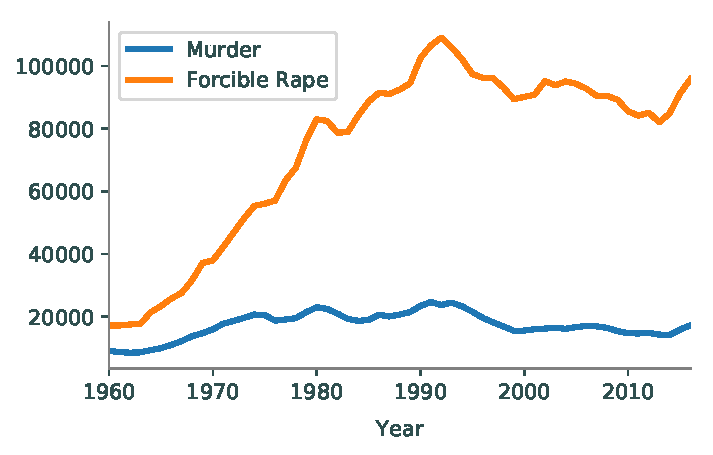
\includegraphics[width=\textwidth]{figures/line_compare.pdf}
\end{subfigure}
%
\begin{subfigure}{.49\textwidth}
    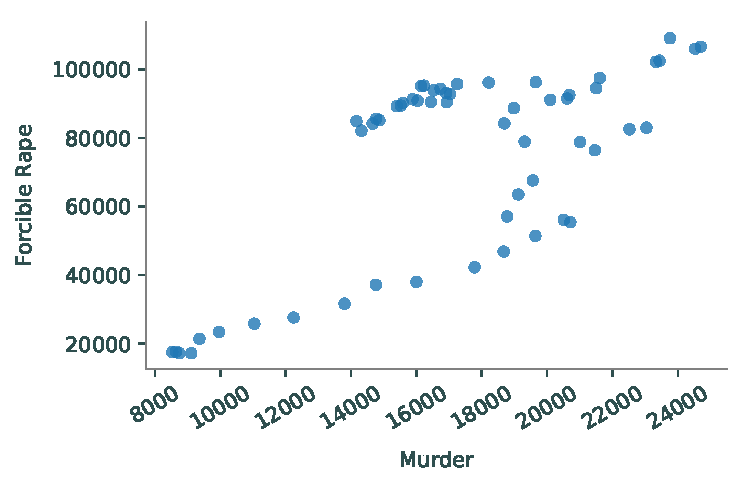
\includegraphics[width=\textwidth]{figures/scatter_compare.pdf}
\end{subfigure}
\end{figure}

What does these graphs show about the data?
First of all, rape is more common than murder.
Second, rates of rape appear to be steadily increased from the mid 1960's to the mid 1990's before leveling out, while murder rates stay relatively constant.
The disparity between rape and murder is confirmed in the scatter plot: the clump of data points at about 15,000 murders and 90,000 rapes shows that there have been many years where rape was relatively high while murder was somewhat low.

\begin{warn}
While analyzing data, especially while searching for patterns and correlations, \textbf{always} ask yourself if the data makes sense and is trustworthy.
What lurking variables could have influenced the data measurements as they were being gathered?

The crime data set is somewhat suspect in this regard.
The murder rate is likely accurate, since murder is conspicuous and highly reported, but what about the rape rate?
Are the number of rapes increasing, or is the percentage of rapes being reported increasing? (It's probably both!)
Be careful about drawing conclusions for sensitive or questionable data.
\end{warn}

Figure \ref{fig:crime-all-v2} also reveals some general patterns relative to time.
For instance, there seems to be a small bump in each type of crime in the early 1980's.
Slicing the entries from 1980 to 1985 provides a closer look.
Since there are only a few entries, we can treat the data as categorical and make a bar chart.

\begin{lstlisting}
# Plot 'Property' and 'Larceny' rates from 1980 to 1985.
>>> crime.loc[1980:1985, ["Property", "Larceny", "Burglary"]].plot(kind="barh",
...                     title="Crime rates from 1980 to 1985")

# Plot the most recent year's crime rates for comparison.
>>> crime.iloc[-1][["Property", "Larceny", "Burglary"]].plot(kind="barh",
...                     title="Crime rates in 2016", color=["C0", "C1", "C2"])
>>> plt.tight_layout()
\end{lstlisting}

\begin{figure}[H] % Plot the early 1980s and the last year.
\captionsetup[subfigure]{justification=centering}
\centering
\begin{subfigure}{.49\textwidth}
    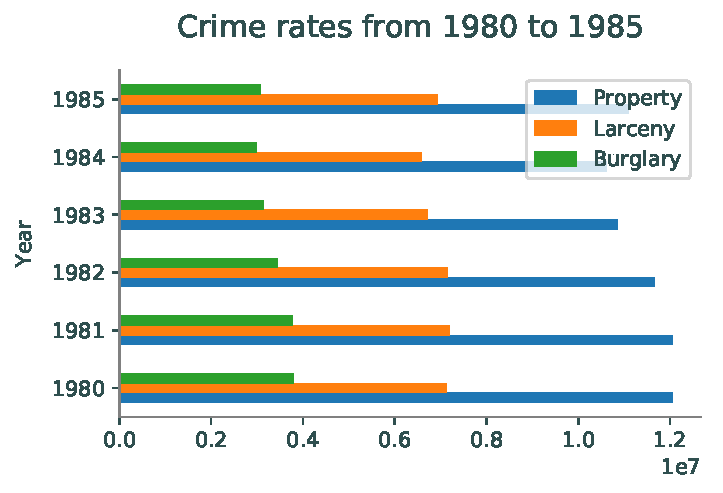
\includegraphics[width=\textwidth]{figures/bar_multi.pdf}
\end{subfigure}
%
\begin{subfigure}{.49\textwidth}
    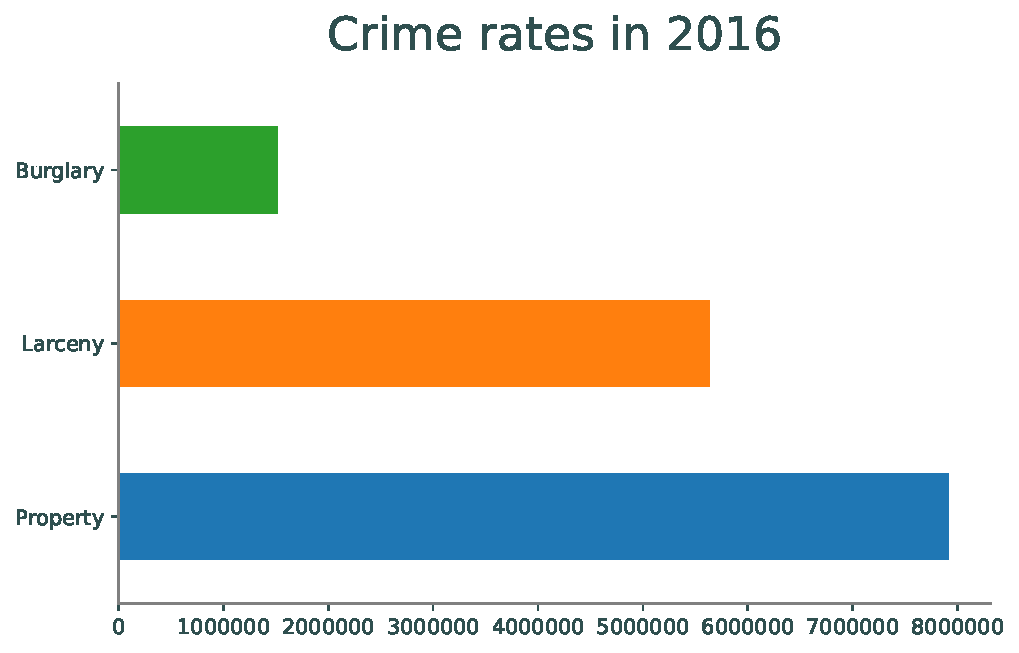
\includegraphics[width=\textwidth]{figures/bar_single.pdf}
\end{subfigure}
\end{figure}

\begin{info} % Use horizontal bar charts.
As a general rule, horizontal bar charts (\li{kind="hbar"}) are better than the default vertical bar charts (\li{kind="bar"}) because most humans can detect horizontal differences more easily than vertical differences.
If the labels are too long to fit on a normal figure, use \li{plt.tight_layout()} to adjust the plot boundaries to fit the labels in.
\end{info}

\section*{Distributional Visualizations} % ====================================

Histograms are good for examining the distribution of a \textbf{single} column in a data set.
While pandas is capable of plotting several histograms on the same plot, the results are usually hard to read.

\begin{lstlisting}
# Plot three histograms together.
>>> crime.plot(kind="hist", y=["Violent", "Vehicle Theft", "Burglary"],
...            bins=20, alpha=.7, rot=30)

# Plot three histograms, stacking one on top of the other.
>>> crime.plot(kind="hist", y=["Violent", "Vehicle Theft", "Burglary"],
...            bins=20, stacked=True, rot=30)
\end{lstlisting}

\begin{figure}[H] % Try to compare histograms.
\captionsetup[subfigure]{justification=centering}
\centering
\begin{subfigure}{.49\textwidth}
    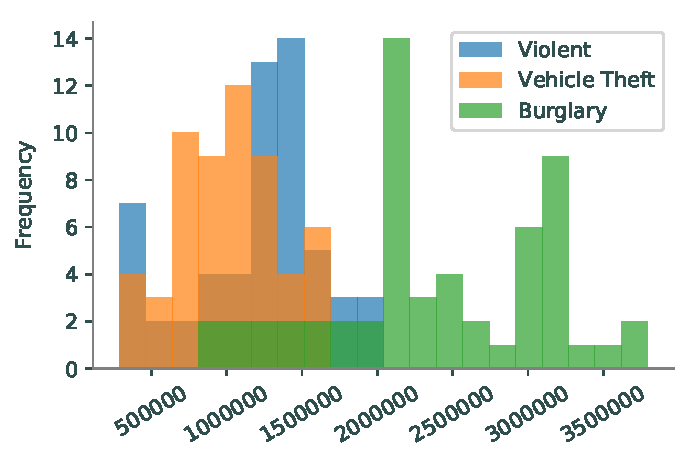
\includegraphics[width=\textwidth]{figures/bad_hist_unstacked.pdf}
\end{subfigure}
%
\begin{subfigure}{.49\textwidth}
    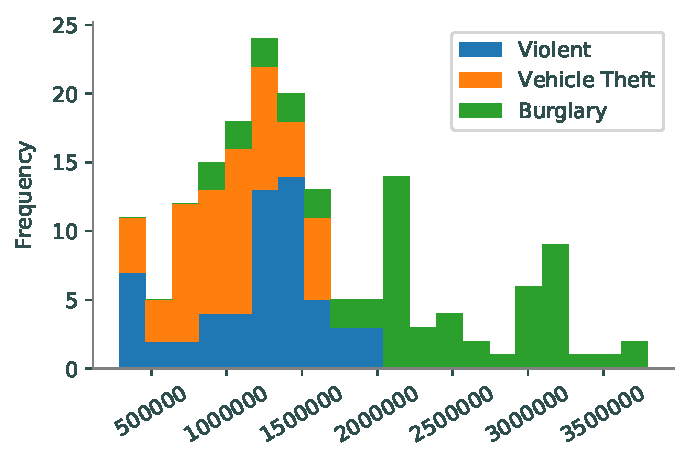
\includegraphics[width=\textwidth]{figures/bad_hist_stacked.pdf}
\end{subfigure}
\end{figure}

Instead of using histograms to compare distributions of data, use box plots.
A \emph{box plot} (sometimes called a ``cat-and-whisker'' plot) shows the five number summary: the minimum, first quartile, median, third quartile, and maximum of the data.
While not quite the same as a histogram, box plots are much better suited to quickly compare relatable distributions.

\begin{lstlisting}
# Compare the distributions of three columns.
>>> crime.plot(kind="box", y=["Violent", "Vehicle Theft", "Burglary"])

# Compare the distributions of all columns but 'Population' and 'Total'.
>>> crime.drop(["Population", "Total"], axis=1).plot(kind="box", vert=False)
\end{lstlisting}

\begin{figure}[H] % Use box plots to compare distributions.
\captionsetup[subfigure]{justification=centering}
\centering
\begin{subfigure}{.49\textwidth}
    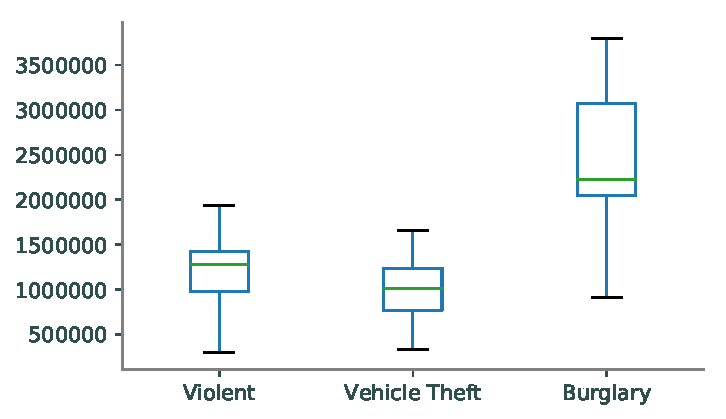
\includegraphics[width=\textwidth]{figures/box_small.pdf}
\end{subfigure}
%
\begin{subfigure}{.49\textwidth}
    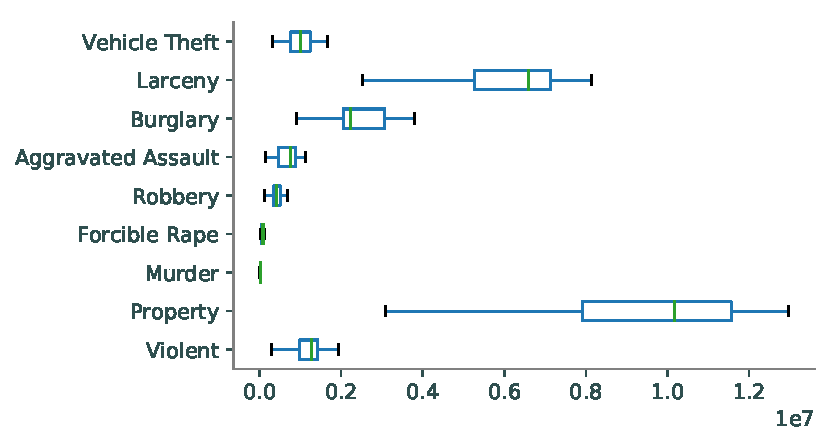
\includegraphics[width=\textwidth]{figures/box_large.pdf}
\end{subfigure}
\end{figure}

% TODO: KDE plot?

% TODO: hexbin plots

% Bar plots, on the other hand, are particularly useful for comparing several categories of data over time, or whenever there is a sense of progression in the index.
% Line plots are better suited to show a more continuous index (such as each year in a century), whereas bar plots are better for a discrete index (a few distinct years).
% Line and bar plots work well when there is a logical progression in the index, such as time.
% However, when frequency of occurrence is more important than the location of the data, histograms and box plots can be more informative.
% Use \li{plot(kind="hist")} to produce a histogram.
% Standard histogram options, such as the number of bins, are also accepted as keyword arguments.
% The \li{alpha} keyword argument makes each bin slightly transparent.

% Sometimes it is helpful to visualize a distribution of values using the box-and-whisker plot which displays the median, first and third quartiles, and outliers.

% Scatter plots are commonly used in a myriad of areas and have a simple implementation in pandas.
% Unlike other plotting commands, \li{scatter} needs both an \li{x} and a \li{y} column as arguments. % TODO: incorporate above!

% The scatter plot option includes many features which can be used to make the plots easier to understand.
% For example, we can change the size of the point based on another column.

\begin{comment} % This should be a pivot table example.
Consider the pydataset \li{HairEyeColor}, which contains the hair and eye color of various individuals.
A scatter plot of hair color vs eye color is relatively useless unless we can see the frequencies with which each combination occurs.
Including the keyword argument \li{s} allows us to control the size of each point.
This can be set to a fixed value or the value in another column.
In the example below, the size of each point is set to the frequency with which each observation occurs.

\begin{lstlisting}
>>> hec = data("HairEyeColor")
>>> X = np.unique(hec["Hair"], return_inverse=True)
>>> Y = np.unique(hec["Eye"], return_inverse=True)
>>> hec["Hair"] = X[1]
>>> hec["Eye"] = Y[1]
>>> hec.plot(kind="scatter", x="Hair", y="Eye", s=hec["Freq"]*10)
>>> plt.xticks([0,1,2,3], X[0])
>>> plt.yticks([0,1,2,3], Y[0])
\end{lstlisting}

\begin{figure}[H]
    \centering
    \includegraphics[width=.7\textwidth]{figures/hair_eye_scatter.pdf}
    \caption{Frequency of Hair-Eye Color Combinations}
\end{figure}
\end{comment}

\subsection*{Hexbin Plots} % --------------------------------------------------

A scatter plot is essentially a plot of samples from the joint distribution of two columns.
However, scatter plots can be uninformative for large data sets when the points in a scatter plot are closely clustered.
\emph{Hexbin plots} solve this problem by plotting point density in hexagonal bins---essentially creating a 2-dimensional histogram.

The file \texttt{sat\_act.csv} contains 700 self reported scores on the SAT Verbal, SAT Quantitative and ACT, collected as part of the Synthetic Aperture Personality Assessment (SAPA) web based personality assessment project.
The obvious question with this data set is ``how correlated are ACT and SAT scores?''
The scatter plot of ACT scores versus SAT Quantitative scores, Figure \ref{fig:pandas-act-scatter}, is highly cluttered, even though the points have some transparency.
A hexbin plot of the same data, Figure \ref{fig:pandas-act-hexbin}, reveals the \textbf{frequency} of points in binned regions.

\newpage

\begin{lstlisting}
>>> satact = pd.read_csv("sat_act.csv", index_col="ID")
>>> list(satact.columns)
<<['gender', 'education', 'age', 'ACT', 'SATV', 'SATQ']>>

# Plot the ACT scores against the SAT Quant scores in a regular scatter plot.
>>> satact.plot(kind="scatter", x="ACT", y="SATQ", alpha=.8)

# Plot the densities of the ACT vs. SATQ scores with a hexbin plot.
>>> satact.plot(kind="Hexbin", x="ACT", y="SATQ", gridsize=20)
\end{lstlisting}

\begin{figure}[H]
\captionsetup[subfigure]{justification=centering}
\centering
\begin{subfigure}{.49\textwidth}
    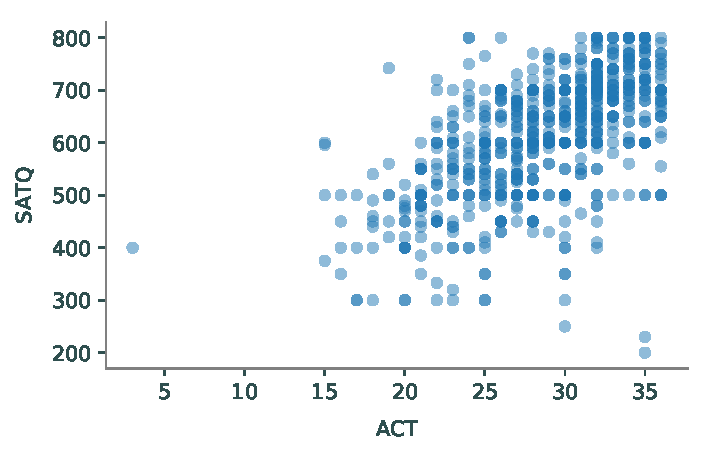
\includegraphics[width=\textwidth]{figures/scores_scatter.pdf}
    \caption{ACT vs. SAT Quant scores.}
    \label{fig:pandas-act-scatter}
\end{subfigure}
%
\begin{subfigure}{.49\textwidth}
    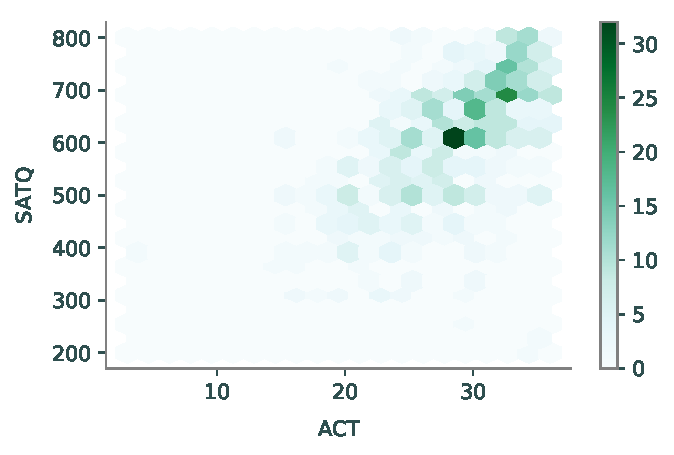
\includegraphics[width=\textwidth]{figures/scores_hexbin.pdf}
    \caption{Frequency of ACT vs. SAT Quant scores.}
    \label{fig:pandas-act-hexbin}
\end{subfigure}
\caption{}
\end{figure}

Just as choosing a good number of \li{bins} is important for a good histogram, choosing a good \li{gridsize} is crucial for an informative hexbin plot.
A large \li{gridsize} creates many small bins and a small \li{gridsize} creates fewer, larger bins.

See \url{http://pandas.pydata.org/pandas-docs/stable/visualization.html} for more types of plots available in Pandas and further examples.

\section*{Principles of Good Data Visualization} % ============================

Visualization is much more than a set of pretty pictures scattered throughout a paper for the sole purpose of providing contrast to the text.
When properly implemented, data visualization is a powerful tool for analysis and communication.
When writing a paper or report, the author must make many decisions about how to use graphics effectively to convey useful information to the reader.
Here we will go over a simple process for making deliberate, effective, and efficient design decisions.

\subsection*{Attention to Detail} % -------------------------------------------

Consider the plot in Figure \ref{fig:nolabels}.
What does it depict?
We can tell from a simple glance that it is a scatter plot of positively correlated data of some kind, with \li{temp}--likely temperature--on the $x$ axis and \li{cons} on the $y$ axis.
However, the picture is not really communicating anything about the dataset.
We have not specified the units for the $x$ or the $y$ axis, we have no idea what \li{cons} is, there is no title, and we don't even know where the data came from in the first place.

\begin{figure}[H]
    \centering
    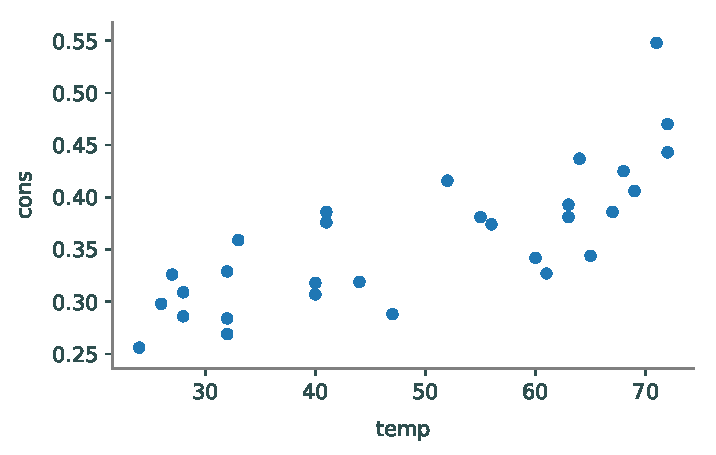
\includegraphics[width=.7\textwidth]{figures/ice_cream_bad.pdf}
    \caption{Non-specific data.}
    \label{fig:nolabels}
\end{figure}

\subsection*{Labels and Citations} % ------------------------------------------

In a homework or lab setting, we sometimes (mistakenly) think that it is acceptable to leave off appropriate labels, legends, titles, and sourcing.
In a published report or presentation, this kind of carelessness is confusing at best and, when the source is not included, even plagiaristic.
Clearly, we need to explain our data in a useful manner that includes all of the vital information.

Consider again Figure \ref{fig:nolabels}.
This figure comes from the \li{Icecream} dataset within the \li{pydataset} package, which we store here in a dataframe and then plot:
\begin{lstlisting}
>>> from pydataset import data
>>> icecream = data("Icecream")
>>> icecream.plot(kind="scatter", x="temp", y="cons")
\end{lstlisting}

We have at this point reproduced the rather substandard plot in Figure \ref{fig:nolabels}.
Using \li{data('Icecream', show\_doc=True)} we find the following information:
\begin{enumerate}
    \item The dataset details ice cream consumption via four-weekly observations from March 1951 to July 1953 in the United States.
    \item \li{cons} corresponds to ``consumption of ice cream per head'' and is measured in pints.
    \item \li{temp} corresponds to temperature, degrees Fahrenheit.
    \item The listed source is: ``Hildreth, C. and J. Lu (1960) \emph{Demand relations with autocorrelated disturbances}, Technical Bulletin No 2765, Michigan State University.''
\end{enumerate}

We add these important details using the following code.
As we have seen in previous examples, pandas automatically generates legends when appropriate.
However, although pandas also automatically labels the $x$ and $y$ axes, our data frame column titles may be insufficient.
Appropriate titles for the $x$ and $y$ axes must also list appropriate units.
For example, the $y$ axis should specify that the consumption is in units of \emph{pints per head}, in place of the ambiguous label \li{cons}.

\begin{lstlisting}
>>> icecream = data("Icecream")
# Set title via the title keyword argument
>>> icecream.plot(kind="scatter", x="temp", y="cons", title="Ice Cream Consumption in the U.S., 1951-1953",)
# Override pandas automatic labelling using xlabel and ylabel
>>> plt.xlabel("Temp (Farenheit)")
>>> plt.ylabel("Consumption per head (pints)")
\end{lstlisting}

To arbitrarily add the necessary text to the figure, use either \li{plt.annotate()} or \li{plt.text()}.
Alternatively, add text immediately below wherever the figure is displayed.

\begin{lstlisting}
>>> plt.text(20, .1, r"Source: Hildreth, C. and J. Lu (1960) \emph{Demand"
...     "relations with autocorrelated disturbances}\nTechnical Bulletin No"
...     "2765, Michigan State University.", fontsize=7)
\end{lstlisting}

Both of these methods are imperfect, however, and can normally be just as easily replaced by a caption attached to the figure in your presentation or document setting.
We again reiterate how important it is that you source any data you use.
Failing to do so is plagiarism.

Finally, we have a clear and demonstrative graphic in Figure \ref{fig:labels}.

\begin{figure}[H]
    \centering
    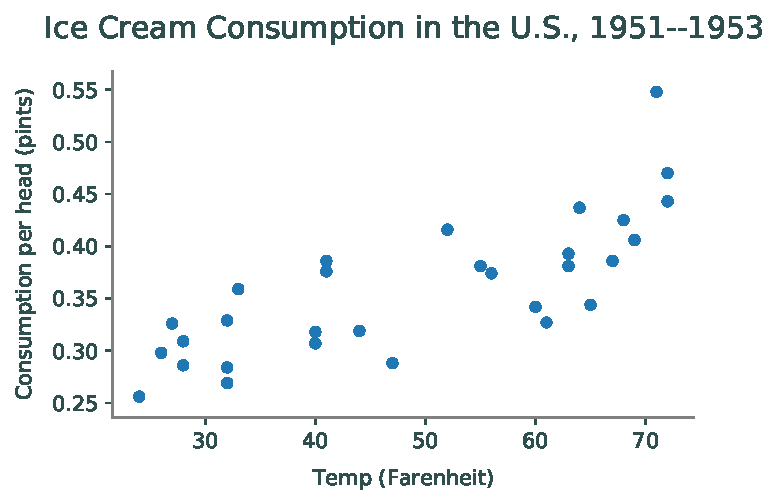
\includegraphics[width=.7\textwidth]{figures/ice_cream_good.pdf}
    \caption{Source:  Hildreth, C. and J. Lu (1960) \emph{Demand relations with autocorrelated disturbances}, Technical Bulletin No 2765, Michigan State University.}
    \label{fig:labels}
\end{figure}

\begin{problem}
The \li{pydataset} module\footnote{Run \texttt{pip install pydataset} if needed.} contains numerous data sets, each stored as a pandas \li{DataFrame}.

\begin{lstlisting}
>>> from pydataset import data

# Call data() to see the entire list of data sets.
# To load a particular data set, enter its ID as an argument to data().
>>> titanic = data("Titanic")
# To see the information about a data set, call data() with show_doc=True.
>>> data("Titanic", show_doc=True)
<<Titanic

PyDataset Documentation (adopted from R Documentation. The displayed
examples are in R)

## Survival of passengers on the Titanic>>
\end{lstlisting}

Visualize and describe at least 5 of the following data sets with 2 or 3 figures each.
Comment on the implications and significance of each visualization and give a comprehensive summary of the data set.

\begin{itemize}
\item \li{"Arbuthnot"}: Ratios of male to female births in London from 1629-1710
\item \li{"trees"}: Girth, height and volume for black cherry trees
\item \li{"road"}: Road accident deaths in the United States
\item \li{"birthdeathrates"}: Birth and death rates by country
\item \li{"bfeed"}: Child breast feeding records
\item \li{"heart"}: Survival of patients on the waiting list for the Stanford heart transplant program
\item \li{"lung"}: Survival in patients with advanced lung cancer from the North Central Cancer Treatment group
\item \li{"birthwt"}: Risk factors associated with low infant birth weight
\item A data set of your choice
\end{itemize}
Include each of the following in each visualization.
\begin{itemize}
\item A clear title, with relevant information for the period or region the data was collected in.
\item Axis labels that specify units.
\item A legend (if appropriate).
\item The source.
You may include the source information in your plot or print it after the plot.
\end{itemize}
\end{problem}
